\item {\bf Semi-supervised EM}

\def\zsi{z^{(i)}}
\def\xsi{x^{(i)}}

Expectation Maximization (EM) is a classical algorithm for unsupervised learning (\emph{i.e.,} learning with hidden or latent variables). In this problem we will explore one of the ways in which the EM algorithm can be adapted to the semi-supervised setting, where we have some labeled examples along with unlabeled examples.

In the standard unsupervised setting, we have $\nexp \in \mathbb{N}$ unlabeled examples $\{x^{(1)},\ldots,x^{(\nexp)}\}$. We wish to learn the parameters of $p(x,z;\theta)$ from the data, but $\zsi$'s are not observed. The classical EM algorithm is designed for this very purpose, where we maximize the intractable $p(x;\theta)$ indirectly by iteratively performing the E-step and M-step, each time maximizing a tractable lower bound of $p(x;\theta)$. Our objective can be concretely written as:

\begin{align*}
    \ell_{\text{unsup}}(\theta) &= \sum_{i=1}^\nexp \log p(\xsi;\theta) \\
    &= \sum_{i=1}^\nexp \log \sum_{\zsi} p(\xsi,\zsi;\theta)
\end{align*}


Now, we will attempt to construct an extension of EM to the semi-supervised setting. Let us suppose we have an \emph{additional} $\tilde{\nexp} \in \mathbb{N}$ labeled examples $\{(\tilde{x}^{(1)},\tilde{z}^{(1)}),\ldots,(\tilde{x}^{(\tilde{\nexp})},\tilde{z}^{(\tilde{\nexp})})\}$ where both $x$ and $z$ are observed. We want to simultaneously maximize the marginal likelihood of the parameters using the unlabeled examples, and full likelihood of the parameters using the labeled examples, by optimizing their weighted sum (with some hyperparameter $\alpha$). More concretely, our semi-supervised objective $\ell_\text{semi-sup}(\theta)$ can be written as:
%
\begin{align*}
    \ell_\text{sup}(\theta) &= \sum_{i=1}^{\tilde{\nexp}} \log p(\tilde{x}^{(i)},\tilde{z}^{(i)};\theta) \\
    \ell_{\text{semi-sup}}(\theta) &= \ell_\text{unsup}(\theta) + \alpha \ell_\text{sup}(\theta)
\end{align*}
%
We can derive the EM steps for the semi-supervised setting using the same approach and steps as before. You are \emph{strongly encouraged} to show to yourself (no need to include in the write-up) that we end up with:

\subsubsection*{E-step (semi-supervised)}

For each $i \in \{1,\ldots,\nexp\}$, set
\begin{align*}
    Q_i^{(t)}(\zsi) := p(\zsi\vert\xsi;\theta^{(t)})
\end{align*}

\subsubsection*{M-step (semi-supervised)}

\begin{align*}
    \theta^{(t+1)} &:= \arg\max_\theta\left[ \sum_{i=1}^\nexp\left( \sum_{\zsi} Q^{(t)}_i(\zsi) \log \frac{ p(\xsi, \zsi;\theta) }{ Q^{(t)}_i(\zsi)}\right)  + \alpha \left(\sum_{i=1}^{\tilde{\nexp}} \log p(\tilde{x}^{(i)},\tilde{z}^{(i)};\theta)\right)\right]
\end{align*}

\begin{enumerate}
  \input{02-semi_supervised_em/01-convergence}

\end{enumerate}


\subsubsection*{Semi-supervised GMM}
Now we will revisit the Gaussian Mixture Model (GMM), to apply our semi-supervised EM algorithm. Let us consider a scenario where data is generated from $k \in \mathbb{N}$ Gaussian distributions, with unknown means $\mu_j \in \R^\di$ and covariances $\Sigma_j \in \mathbb{S}_+^\di$ where $j \in \{1,\ldots,k\}$. We have $\nexp$ data points $\xsi \in \R^\di, i \in \{1,\ldots,\nexp\}$, and each data point has a corresponding latent (hidden/unknown) variable $\zsi \in \{1,\ldots,k\}$ indicating which distribution $\xsi$ belongs to. Specifically, $\zsi \sim \text{Multinomial}(\phi)$, such that $\sum_{j=1}^k\phi_j = 1$ and $\phi_j \ge 0$ for all $j$, and $\xsi\vert\zsi \sim \mathcal{N}\left(\mu_{\zsi}, \Sigma_{\zsi}\right)$ i.i.d. So, $\mu$, $\Sigma$, and $\phi$ are the model parameters.

We also have additional $\tilde{\nexp}$ data points $\tilde{x}^{(i)} \in \R^\di, i \in \{1,\ldots,\tilde{\nexp}\}$, and an associated \emph{observed} variable $\tilde{z}^{(i)} \in \{1,\ldots,k\}$ indicating the distribution $\tilde{x}^{(i)}$ belongs to. Note that $\tilde{z}^{(i)}$ are known constants (in contrast to $\zsi$ which are unknown \emph{random} variables). As before, we assume $\tilde{x}^{(i)}\vert \tilde{z}^{(i)} \sim \mathcal{N}\left(\mu_{\tilde{z}^{(i)}}, \Sigma_{\tilde{z}^{(i)}}\right)$ i.i.d.


In summary we have $\nexp$ + $\tilde{\nexp}$ examples, of which $\nexp$ are unlabeled data points $x$'s with unobserved $z$'s, and $\tilde{\nexp}$ are labeled data points $\tilde{x}^{(i)}$ with corresponding observed labels $\tilde{z}^{(i)}$. The traditional EM algorithm is designed to take only the $\nexp$ unlabeled examples as input, and learn the model parameters $\mu$, $\Sigma$, and $\phi$.


Our task now will be to apply the semi-supervised EM algorithm to GMMs in order to also leverage the additional $\tilde{\nexp}$ labeled examples, and come up with semi-supervised E-step and M-step update rules specific to GMMs. Whenever required, you can cite the lecture notes for derivations and steps.


\begin{enumerate}
  \setcounter{enumii}{1}
  \input{02-semi_supervised_em/02-e-step}
  \input{02-semi_supervised_em/03-m-step}
  \item \points{2d}
\textbf{Classical (Unsupervised) EM Implementation.}
For this sub-question, we are only going to consider the $\nexp$ unlabeled examples. Follow the instructions in |src-semi_supervised_em/submission.py| to implement the traditional EM algorithm, and run it on the unlabeled data-set until convergence.
More specifically, please complete the |main| and |run_em| functions. Note: feel free to create your own helper functions in the development of your solution.

Autograder test case |2d-1-basic| can be used to verify a correct implementation. Before running the test case, change line 92 to |skip = False| (this test is skipped by default to make the autograder faster).  It will run three trials and use the provided plotting function to construct a scatter plot of the resulting assignments to clusters (one plot for each trial). The output plot will indicate cluster assignments by assigning unique colors for each cluster (\emph{i.e.,} the cluster which had the highest probability in the final E-step).  Do not submit these plots; they are not graded.\\

Your plots should look similar to the following:

  \begin{figure}[H]
    \centering
    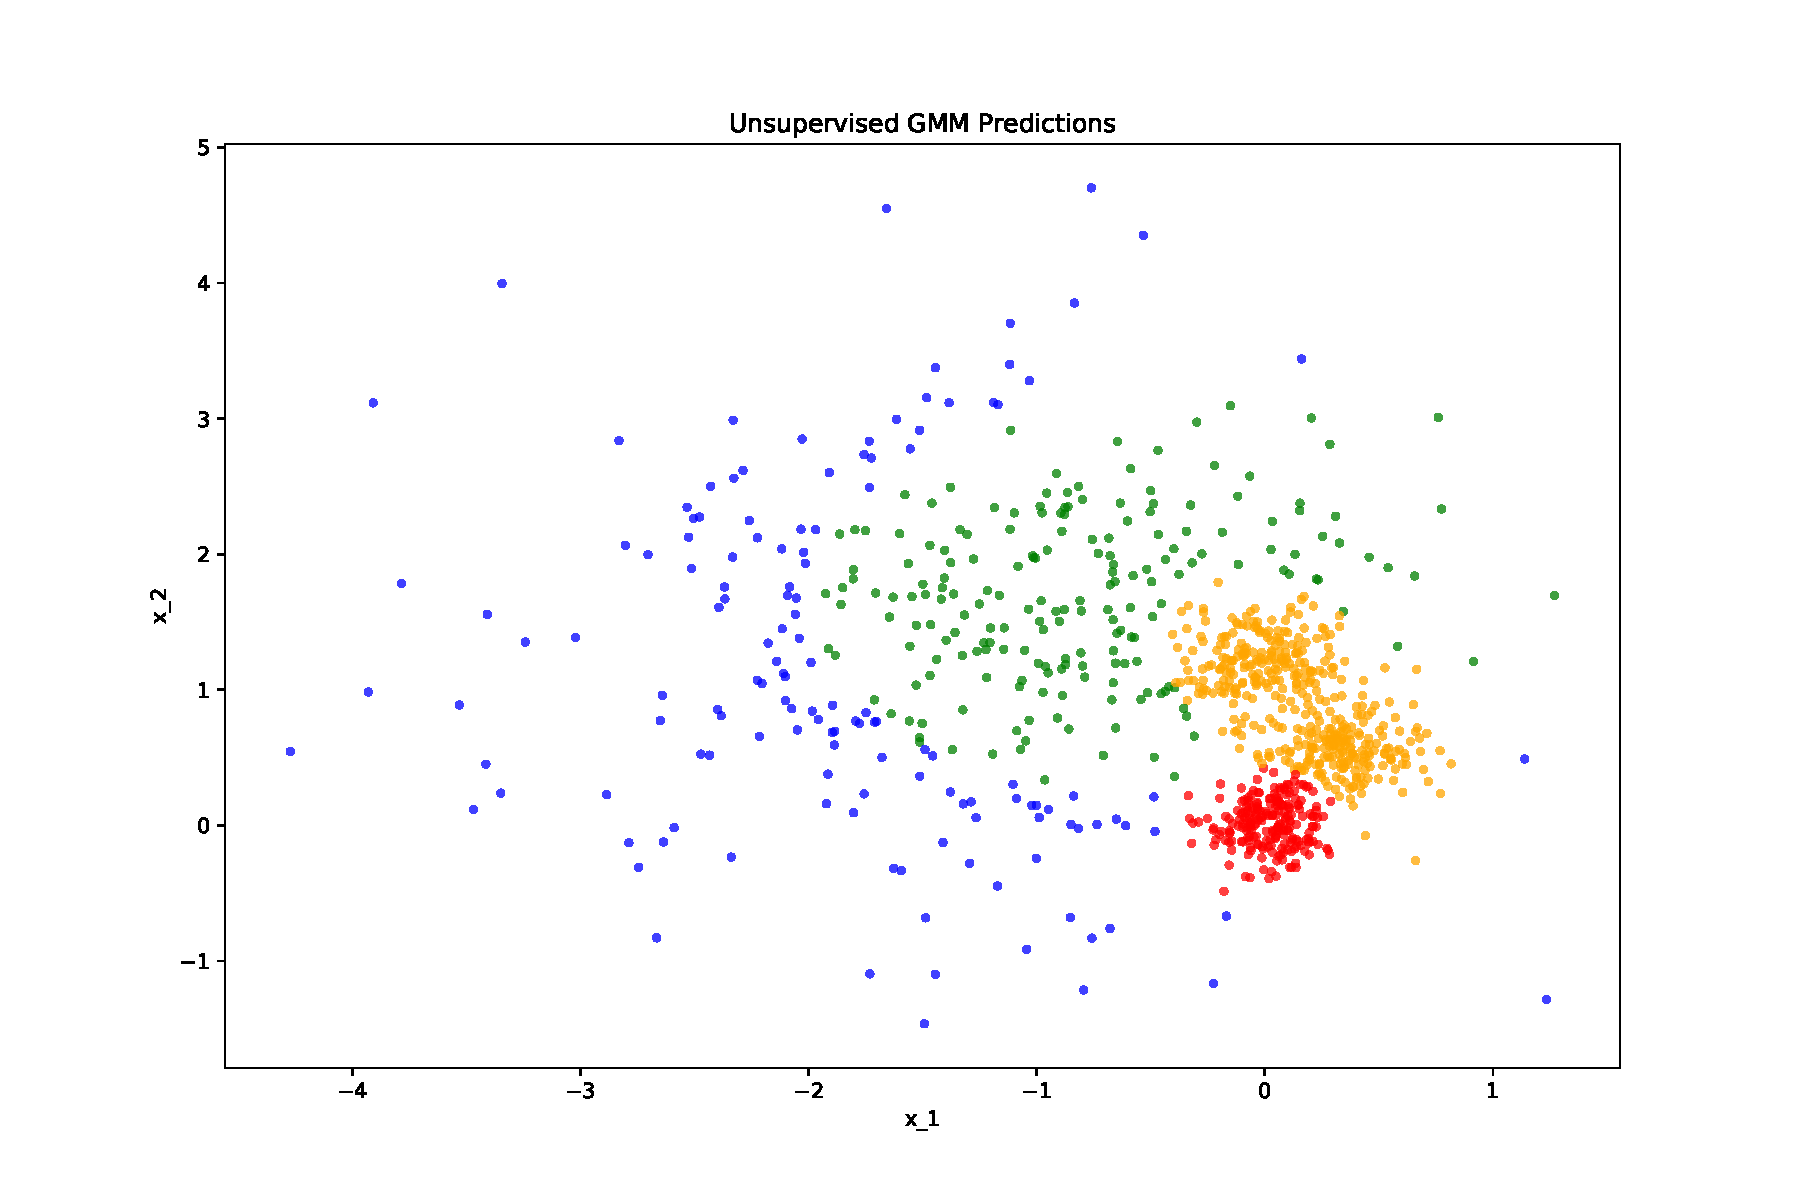
\includegraphics[width=0.3\textwidth]{02-semi_supervised_em/pred_0.pdf}
    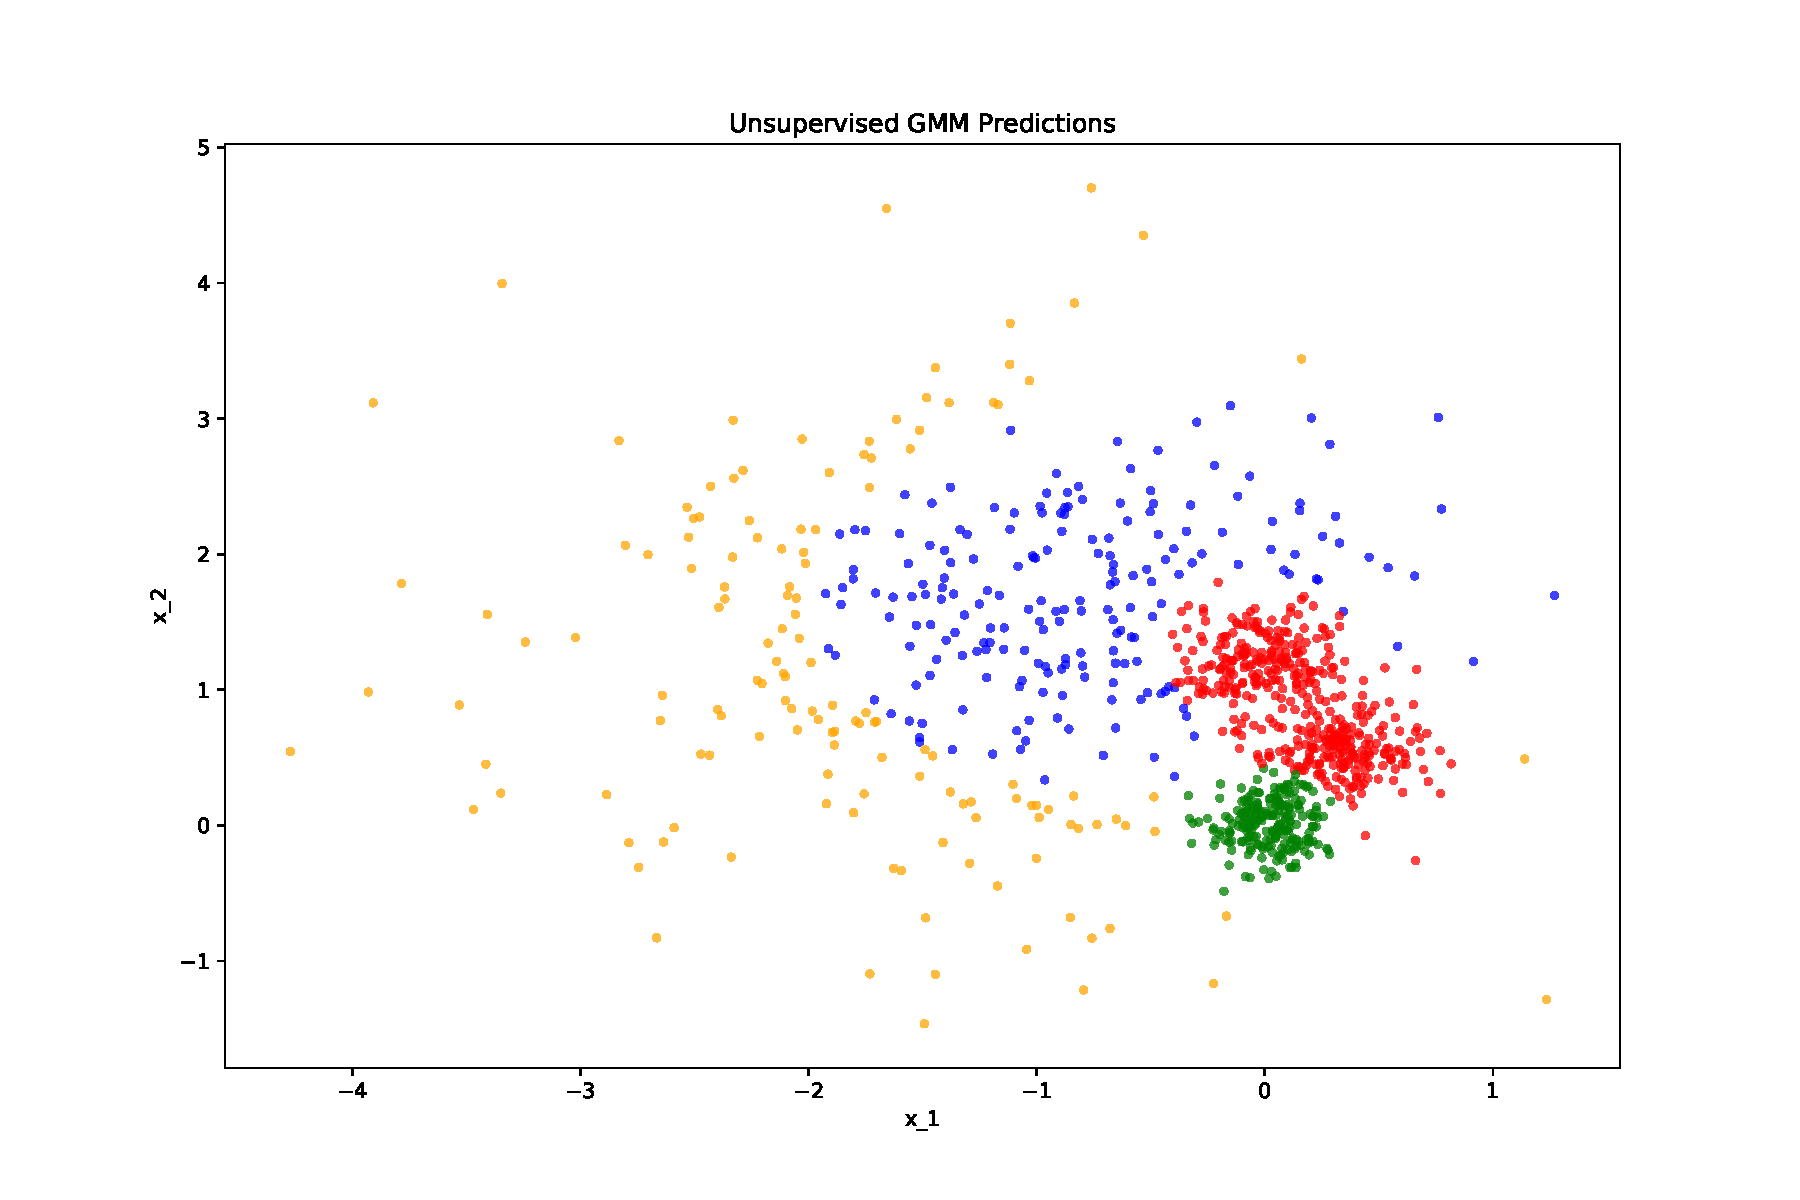
\includegraphics[width=0.3\textwidth]{02-semi_supervised_em/pred_1.pdf}
    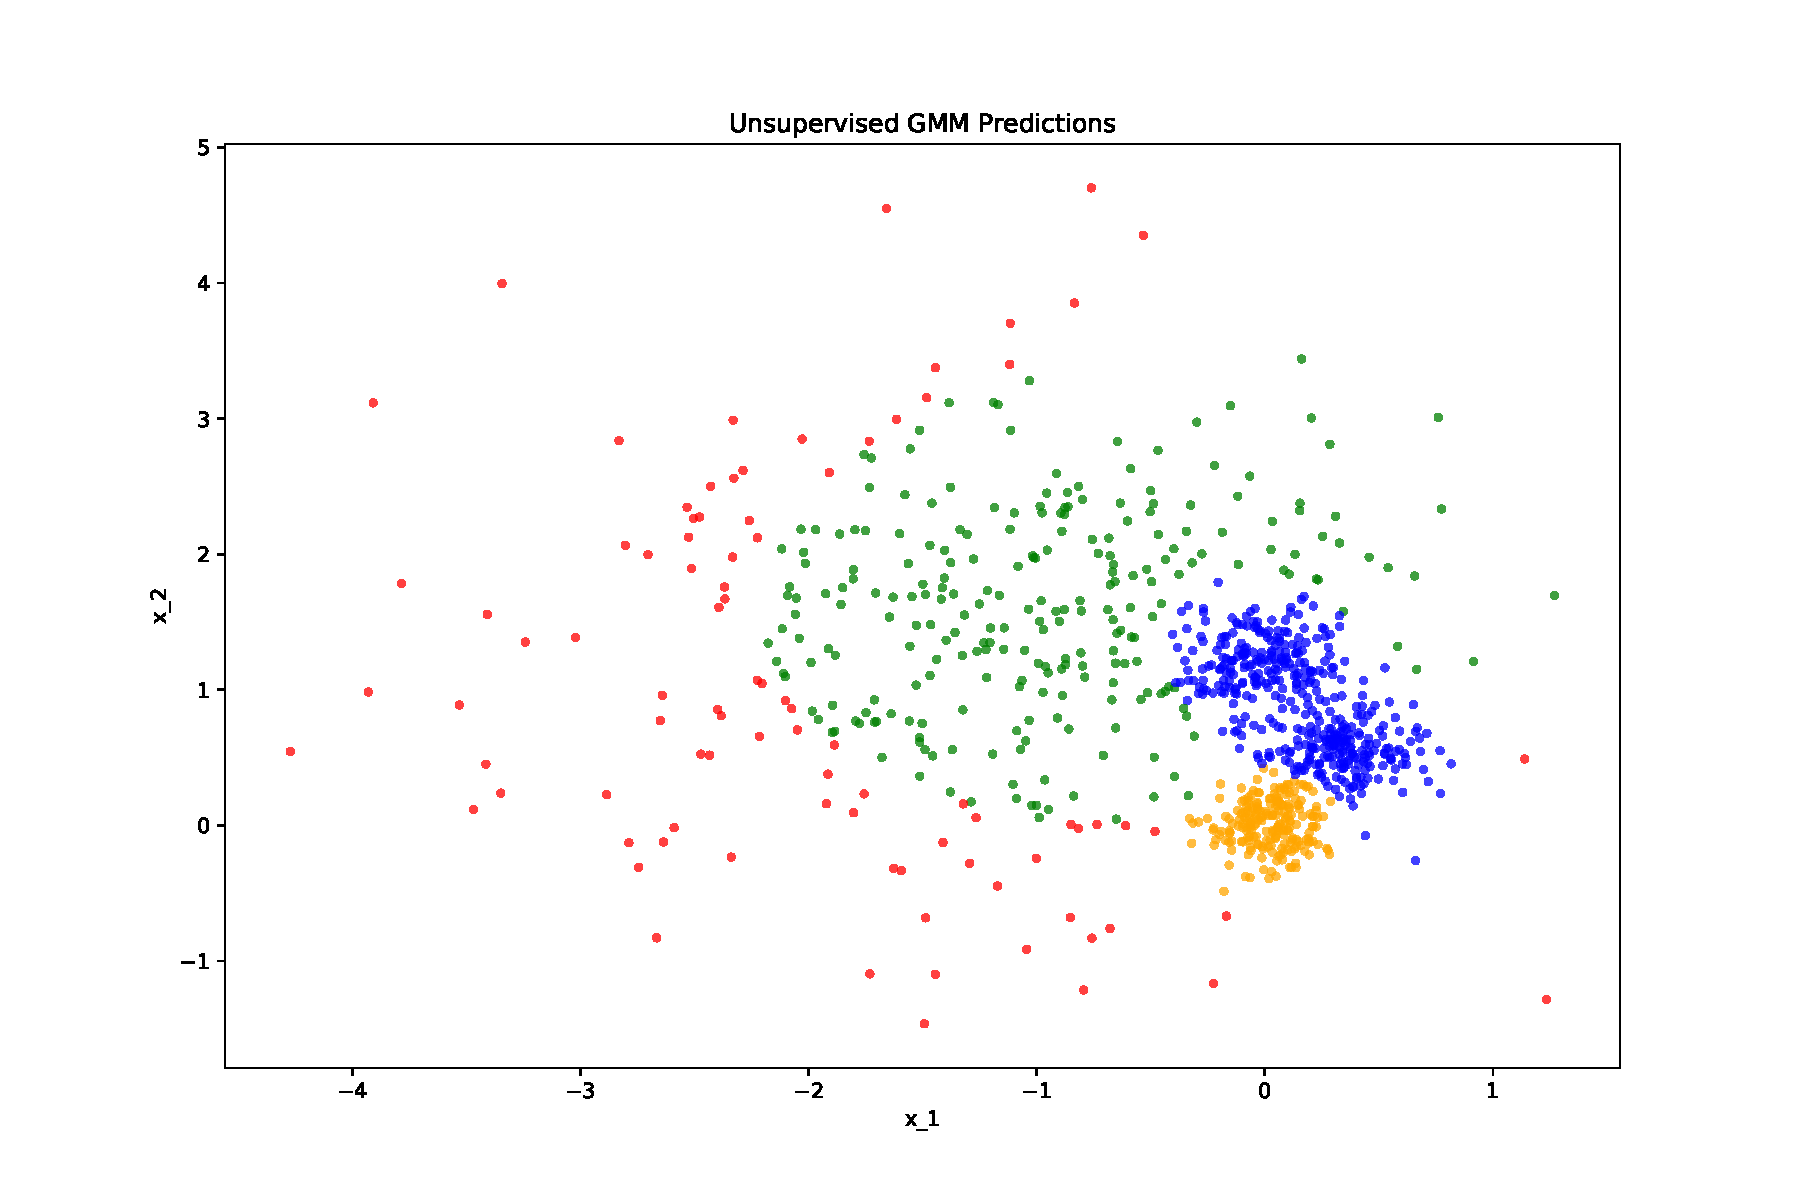
\includegraphics[width=0.3\textwidth]{02-semi_supervised_em/pred_2.pdf}
    \caption{Predictions made by GMM model with unsupervised EM. Visual impaired students can access the corresponding desmos plots \href{https://www.desmos.com/calculator/y0yq8ahnvk}{here}, \href{https://www.desmos.com/calculator/leymlqxcql}{here} and \href{https://www.desmos.com/calculator/open1qetjj}{here}}
  \end{figure}

  \item \points{2e}
\textbf{Semi-supervised EM Implementation.}
Now we will consider both the labeled and unlabeled examples (a total of $\nexp + \tilde{\nexp}$), with 5 labeled examples per cluster. We have provided starter code for splitting the dataset into matrices \texttt{x} and \texttt{x\_tilde} of unlabeled and labeled examples respectively. Add to your code in |src-semi_supervised_em/submission.py| to implement the modified EM algorithm, and run it on the dataset until convergence.
More specifically, you will complete the |main| and |run_semi_supervised_em| functions. Note: feel free to create your own helper functions in the development of your solution.

Autograder test case |2e-1-basic| can be used to verify a correct implementation.  Before running the test case, change line 143 to |skip = False| (this test is skipped by default to make the autograder faster).  It will runcreate a plot for each trial, as done in the previous sub-question.

Your plots should look similar to the following (your plots are not graded):

  \begin{figure}[H]
    \centering
    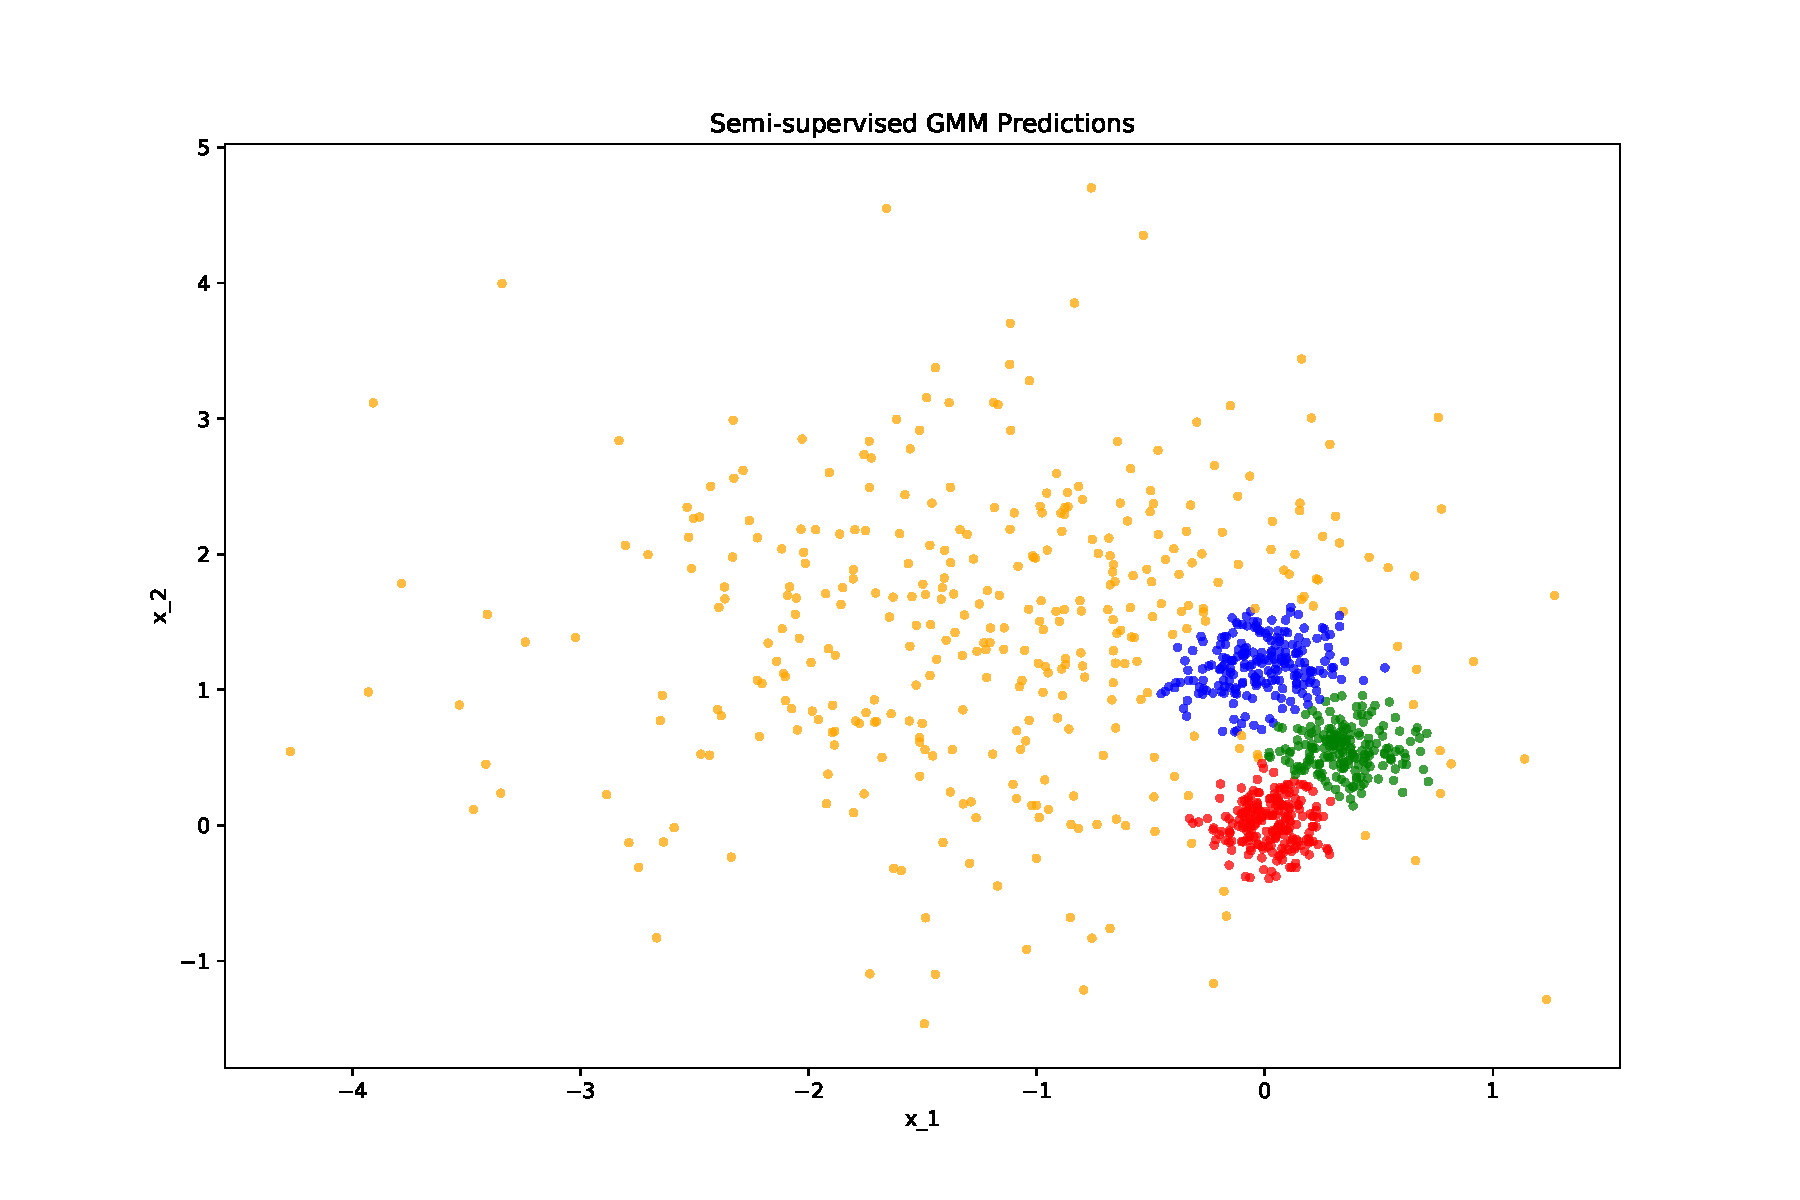
\includegraphics[width=0.3\textwidth]{02-semi_supervised_em/pred_ss_0.pdf}
    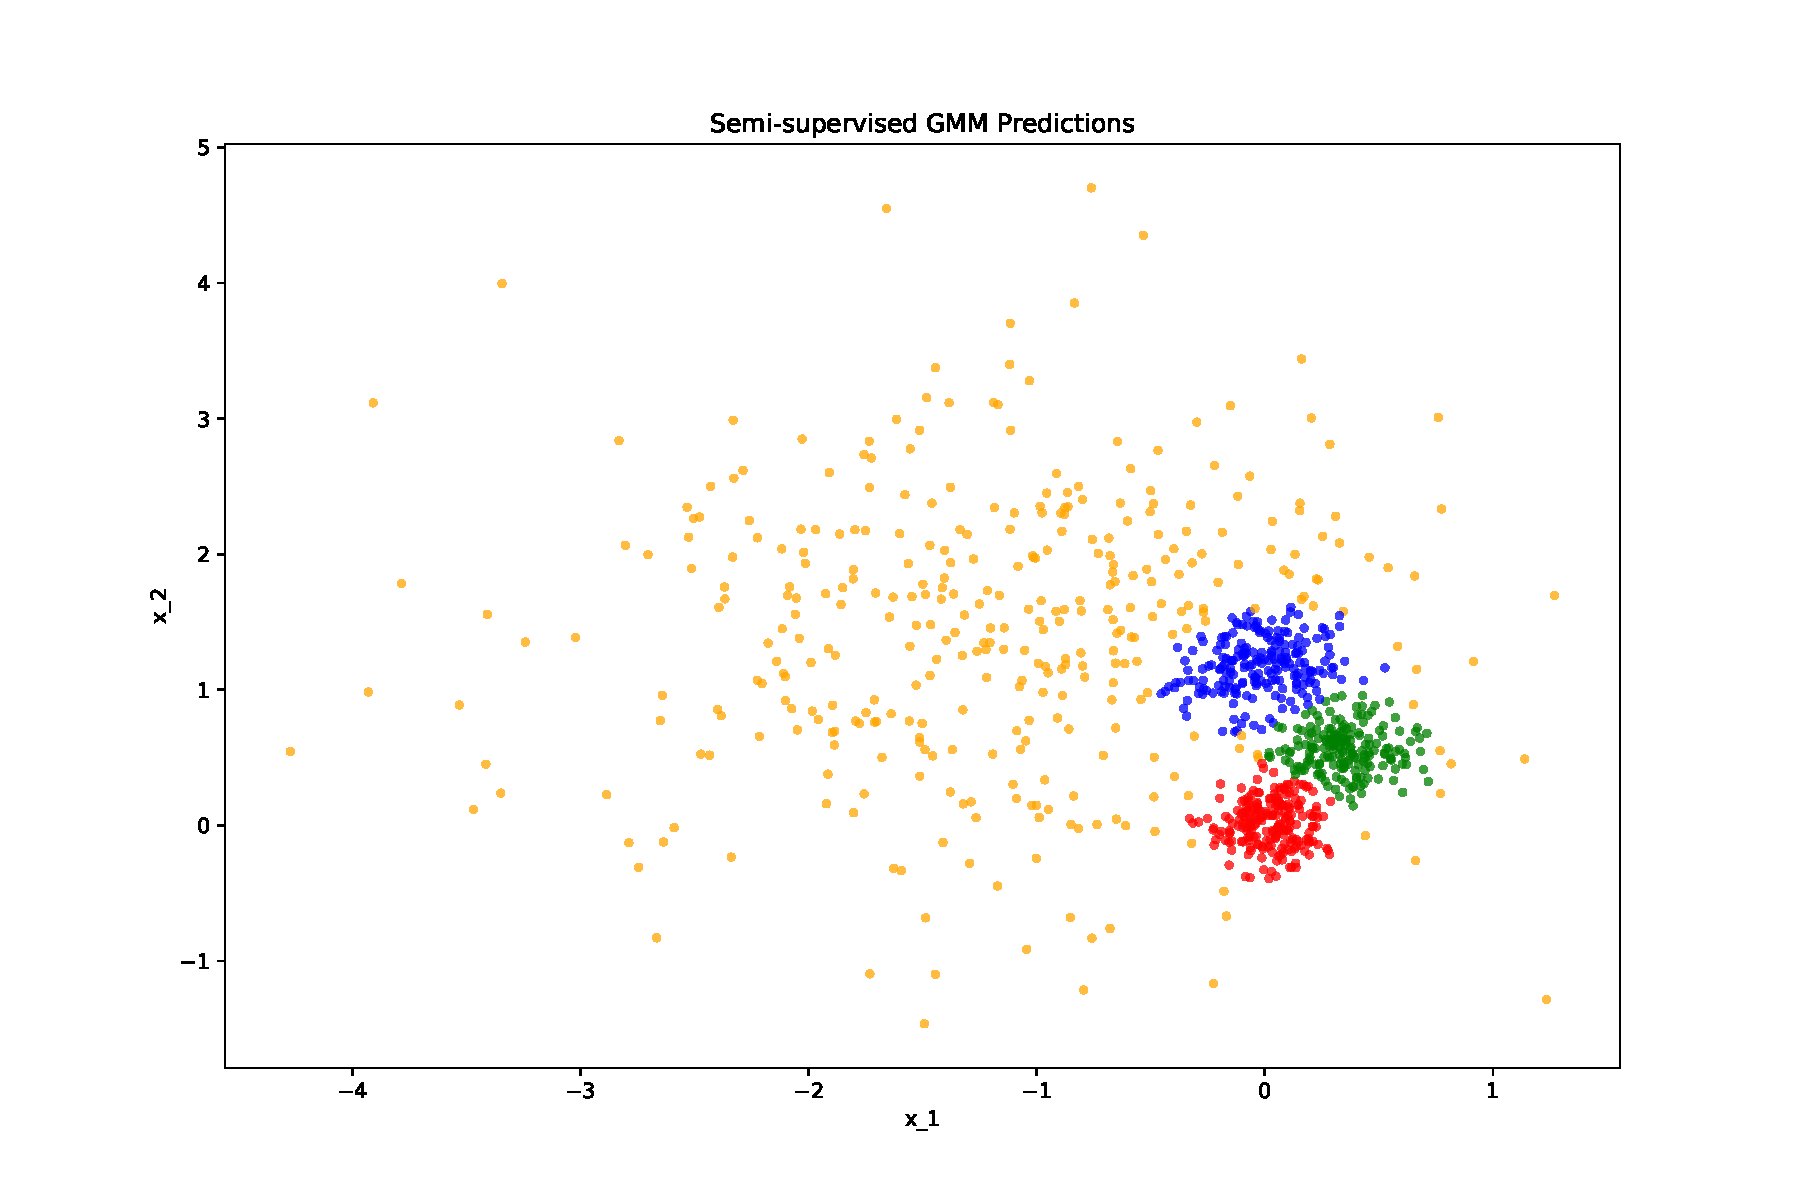
\includegraphics[width=0.3\textwidth]{02-semi_supervised_em/pred_ss_1.pdf}
    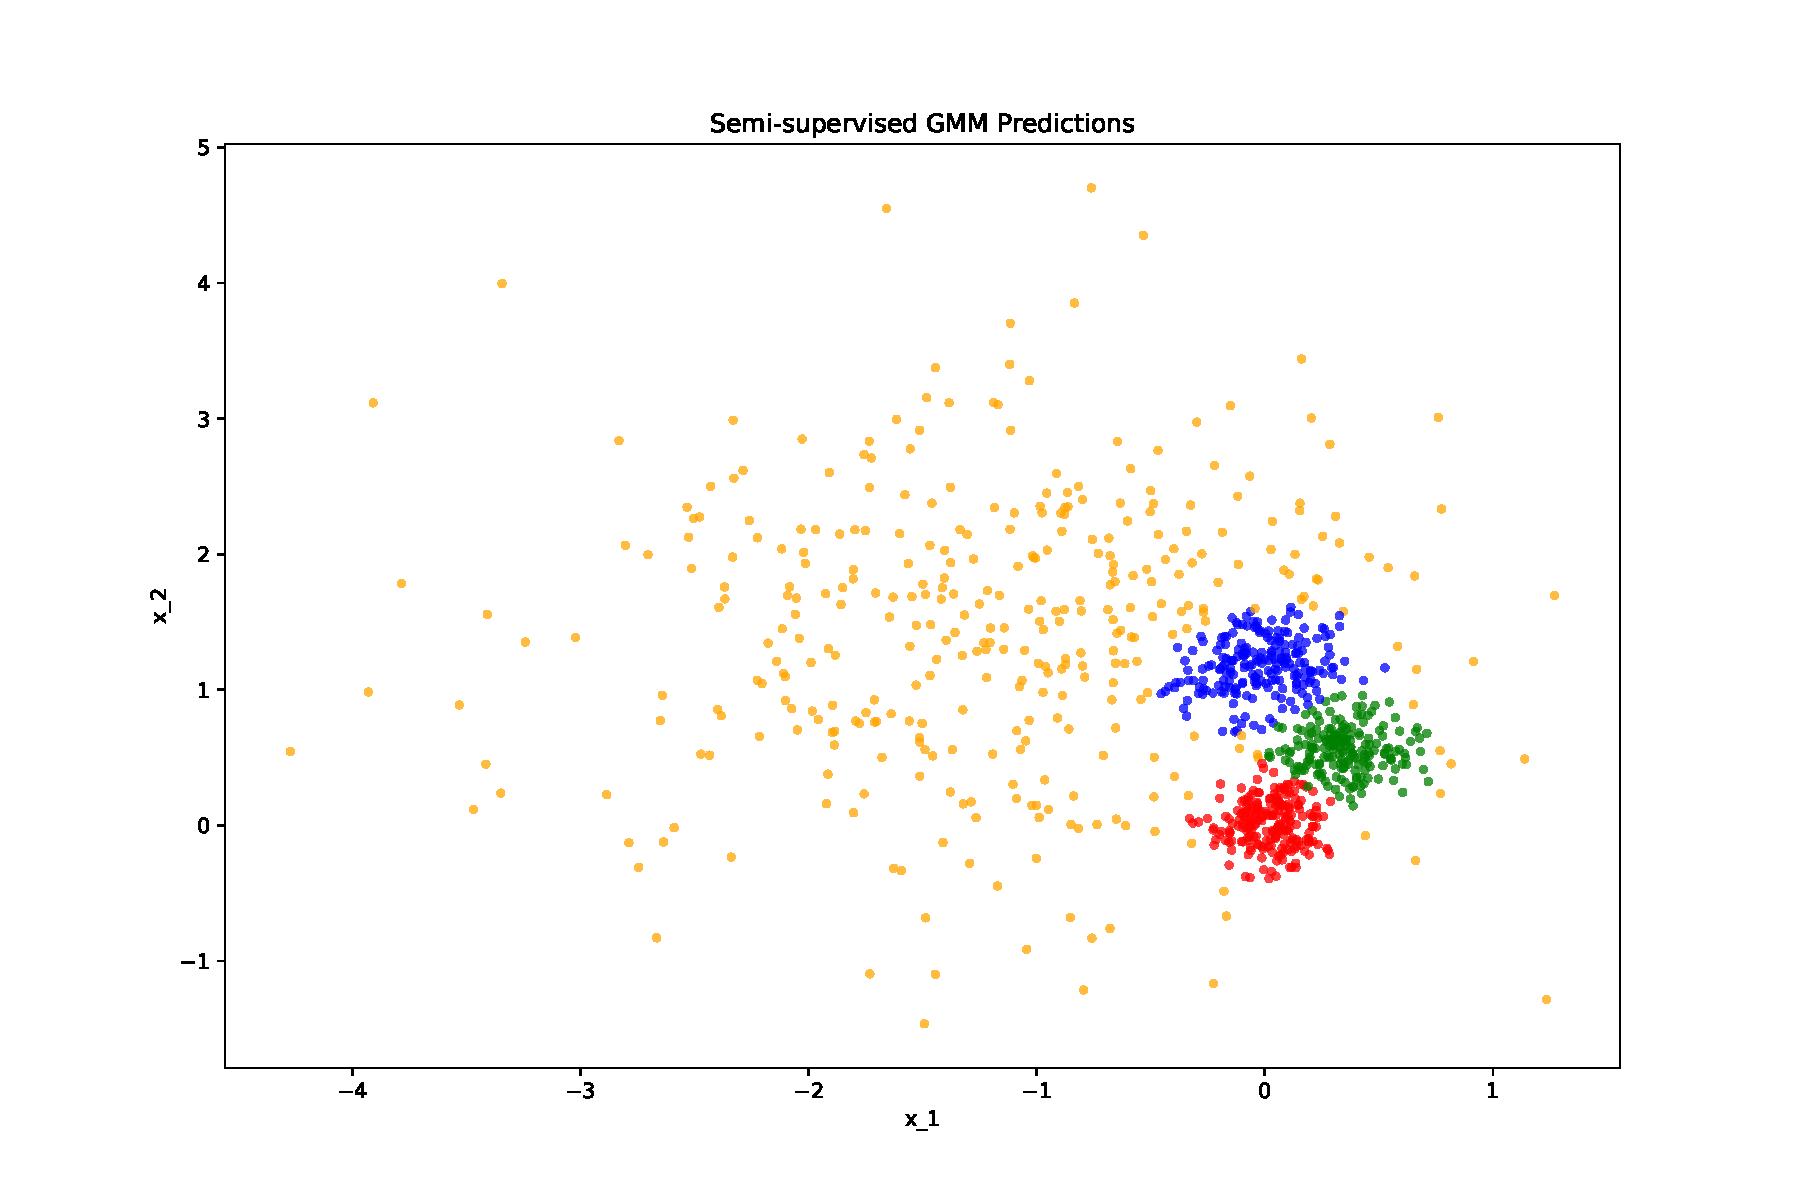
\includegraphics[width=0.3\textwidth]{02-semi_supervised_em/pred_ss_2.pdf}
    \caption{Predictions made by GMM model with semi-supervised EM. Visual impaired students can access the corresponding desmos plots \href{https://www.desmos.com/calculator/fyu9j2vtbp}{here}, \href{https://www.desmos.com/calculator/yxtvpmgwbk}{here} and \href{https://www.desmos.com/calculator/nr7tybpdho}{here}}
  \end{figure}

  \input{02-semi_supervised_em/06-comparison}
\end{enumerate}
